\documentclass[11pt]{article}

\usepackage[margin=1in]{geometry}
\usepackage{amsmath,amssymb}
\usepackage{booktabs}
\usepackage{graphicx}
\usepackage{url}
\usepackage{xurl}
\usepackage{array}
\usepackage{tabularx}
\usepackage{microtype}
\usepackage{xcolor}
\usepackage{tikz}
\usepackage{hyperref}
\usetikzlibrary{arrows.meta,positioning,calc,fit,shapes.geometric,backgrounds}
% Shared figure macro file for ODCR paper figures.
% Chat owns figure design and semantics. Codex may update paths and apply
% exact Chat-authored TikZ/LaTeX replacements, then fix compile-only issues.

\tikzset{
  odcrPanel/.style={draw=gray!45, rounded corners=3pt, inner sep=5pt},
  odcrArrow/.style={-{Stealth[length=2mm]}, thick},
  odcrDashedArrow/.style={-{Stealth[length=2mm]}, thick, dashed, draw=gray!70}
}


\emergencystretch=2em

\hypersetup{
  colorlinks=true,
  linkcolor=blue,
  citecolor=blue,
  urlcolor=blue
}

\title{ODCR: Reliability-Gated Dynamic Causal Refinement for Cross-Domain Explainable Recommendation}
\author{Anonymous Authors}
\date{}

\begin{document}

\maketitle

\begin{abstract}
Cross-domain explainable recommendation must predict target-domain preferences
and generate explanations that remain content-specific, domain-appropriate, and
faithful to recommendation evidence. A central failure mode is explanation
degeneration, where generators learn self-reinforcing textual shortcuts instead
of user--item rationale. Building on D4C, which diagnoses degeneration as a
dynamic feedback process \(W^{(t)} \rightarrow E^{(t)} \rightarrow
W^{(t+1)}\), ODCR refines the coarse textual attribute \(W^{(t)}\) into stable
content evidence \(C\), feedback-sensitive hierarchical style \(S^{(t)}\), and
counterfactual reliability \(R_{cf}\). This refinement yields a complete
control loop: evidence-anchored content/style decomposition, hierarchical style
state modeling, reliability-gated counterfactual routing, and controlled
faithful explanation generation. ODCR therefore learns explanations from
\(P(E\mid U,I,C,S,R_{cf})\) rather than shortcut dependence on \(P(E\mid W)\).
We report current single-run results on four directed transfer settings,
treating them as bounded evidence for the proposed dynamic causal refinement
rather than as a multi-seed benchmark-dominance claim.
\end{abstract}

\section{Introduction}

Explainable recommendation asks a system to predict user preferences and to
justify those predictions with natural-language explanations
\cite{explainable_rec_survey}. In cross-domain settings this problem becomes
especially fragile: evidence can transfer across domains, but review
conventions, item vocabularies, and explanation styles can shift at the same
time \cite{crossdomain_survey}. A generator that appears fluent in the target
domain may still produce explanations that are generic, repetitive, or weakly
connected to the user--item evidence. We refer to this failure mode as
explanation degeneration.

D4C provides the closest causal foundation for this problem \cite{d4c}. Its
key insight is not only that hidden textual attributes \(W\) can act as
domain-level shortcuts, but that these shortcuts participate in a dynamic
feedback process. Textual attributes at time \(t\) influence explanations, and
generated or observed explanations can reshape future textual attributes:
\[
  W^{(t)} \rightarrow E^{(t)} \rightarrow W^{(t+1)} .
\]
This dynamic view explains why degeneration can be self-reinforcing. Ordinary
generators can learn a shortcut from \(W^{(t)}\) to \(E^{(t)}\), preserving
domain-looking language while weakening the genuine user--item interaction
path that should support an explanation.

ODCR builds on this dynamic feedback diagnosis. Its starting point is that a
single coarse textual variable \(W^{(t)}\) is too broad for controlled
explanation learning. The variable mixes at least three forces: stable content
evidence, feedback-sensitive expression style, and the reliability of
counterfactual evidence. ODCR therefore refines the D4C textual-feedback view
as
\[
  W^{(t)} \Rightarrow (C, S^{(t)}, R_{cf}),
\]
where \(C\) denotes stable content evidence, \(S^{(t)}\) denotes a dynamic
hierarchical style state, and \(R_{cf}\) denotes the reliability with which
counterfactual evidence should influence learning. The resulting method is not
an engineering-stage pipeline. It is a reliability-gated dynamic causal control
framework for cross-domain explainable recommendation.

\begin{figure}[t]
  \centering
  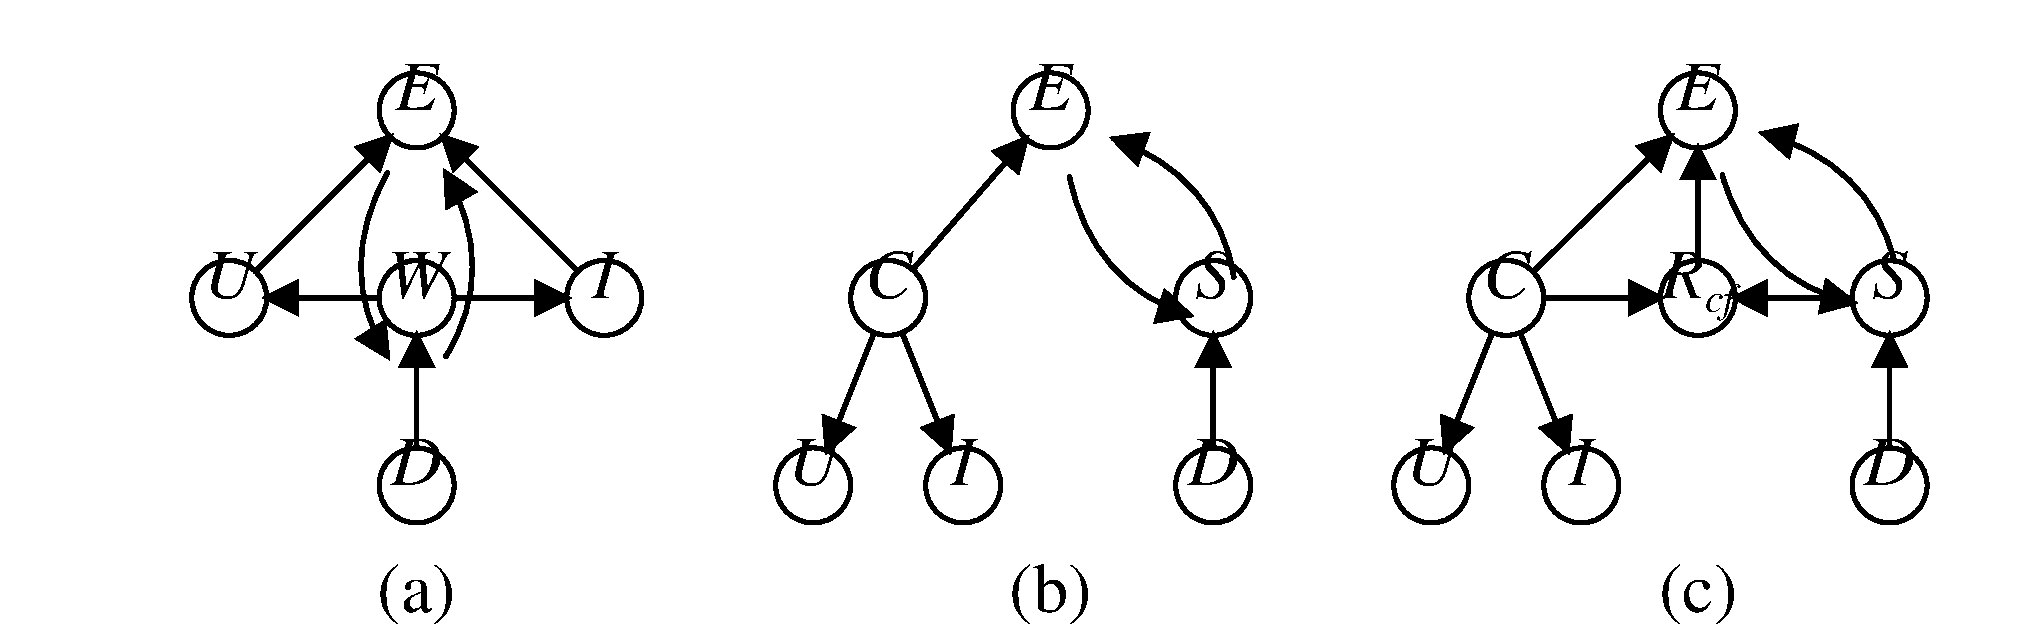
\includegraphics[width=\textwidth]{figures/figure1_dynamic_causal_refinement.pdf}
  \caption{Dynamic causal refinement from D4C to ODCR. D4C explains explanation degeneration as a feedback loop between contextual textual attributes and explanations. ODCR refines this loop into stable content evidence, feedback-sensitive hierarchical style, and counterfactual reliability control.}
  \label{fig:causal_refinement}
\end{figure}

Figure~\ref{fig:causal_refinement} summarizes the refinement. ODCR first
anchors content/style decomposition in evidence, so that content \(C\) captures
what should be explained while style \(S^{(t)}\) captures how the explanation
is expressed. It then models style hierarchically as a domain-global state plus
instance-local residual, localizing dynamic feedback to style rather than
allowing feedback to overwrite content. Counterfactual examples are further
filtered and weighted by \(R_{cf}\), so unreliable shifts do not dominate
learning. Finally, the explanation generator is conditioned on
\((U,I,C,S,R_{cf})\), with faithfulness alignment keeping generated content
consistent with rating-relevant evidence.

This manuscript makes four contributions:
\begin{itemize}
  \item \textbf{Dynamic causal refinement.} ODCR builds on D4C's dynamic
  textual-feedback diagnosis and refines coarse textual attributes into
  controllable variables for content, style, and counterfactual reliability.
  \item \textbf{Evidence-anchored decomposition.} ODCR separates stable
  content evidence from feedback-sensitive domain style, avoiding an
  undifferentiated textual shortcut.
  \item \textbf{Reliability-gated counterfactual control.} ODCR filters,
  routes, and weights counterfactual evidence using reliability and
  uncertainty-aware signals.
  \item \textbf{Controlled faithful generation.} ODCR generates explanations
  conditioned on content, style, and reliability-controlled evidence while
  keeping explanation content aligned with rating-relevant evidence.
\end{itemize}

\section{Related Work}

\subsection{Generative Explainable Recommendation and Degeneration}

Explainable recommendation studies models that pair recommendation decisions
with textual or structured rationales \cite{explainable_rec_survey}. Neural
and language-model-based systems such as PETER, PEPLER, ReXPlug, ERRA, and
AdaReX demonstrate that explanations can be generated jointly with
recommendation signals \cite{peter,pepler,rexplug,erra,adarex}. These models
also highlight the central risk for this paper: fluent explanations are not
automatically faithful explanations. When a generator overuses common review
phrases or domain templates, explanation quality degenerates even if the text
looks plausible.

\subsection{Cross-Domain Explainable Recommendation}

Cross-domain recommendation transfers evidence from a source domain to a
target domain \cite{crossdomain_survey}. Cross-domain explainable
recommendation adds a second transfer problem: the explanation must preserve
recommendation content while adapting to target-domain language. This makes
content and style inseparable if the model treats text as one coarse signal.
ODCR addresses this by representing content evidence and style state as
separate control variables rather than relying on a single domain-level
textual attribute.

\subsection{Causal and Counterfactual Recommendation}

D4C is the closest causal foundation for ODCR \cite{d4c}. It diagnoses
cross-domain explanation degeneration through hidden textual attributes \(W\)
and uses domain counterfactual reasoning to reduce shortcut dependence. ODCR
inherits this causal view but emphasizes the dynamic feedback part of the
diagnosis: \(W^{(t)}\) influences explanations, and explanations can feed back
into future textual attributes. ODCR refines this process into stable content
evidence \(C\), dynamic style \(S^{(t)}\), and reliability-gated
counterfactual influence \(R_{cf}\).

\subsection{Controlled Generation, Faithfulness, and Consistency}

Controlled explanation generation requires more than producing text in the
right domain style. The generated explanation should remain tied to the
content evidence that supports the recommendation. ODCR therefore positions
controlled generation and faithfulness alignment as output-side parts of the
method: \(C\) controls what is said, \(S^{(t)}\) controls how it is expressed,
and \(R_{cf}\) controls which counterfactual signals are trusted during
learning. Modern external systems such as CIER, MAPLE, ELIXIR, Prism, and XRec
remain comparison targets once adapted to the same data and evaluation setting;
the current manuscript does not claim results against them.

\section{Method}

\subsection{Problem Formulation}

Let \(\mathcal{D}_s\) and \(\mathcal{D}_t\) denote a source domain and a target
domain. Each domain contains user--item interaction records
\((u,i,r,e)\), where \(u\) is a user, \(i\) is an item, \(r\) is an observed
rating, and \(e\) is a natural-language explanation or review-derived
explanation target. Given source-domain evidence and target-domain evidence,
the goal is to predict a target-domain rating \(\hat r_{ui}\) and generate a
target-domain explanation \(\hat e_{ui}\) for a user--item pair.

The target explanation should satisfy two constraints. First, it should be
content-grounded: the explanation should describe evidence relevant to the
user and item rather than generic domain text. Second, it should be
domain-appropriate: the explanation should use target-domain expression style
without allowing style to replace recommendation evidence. ODCR formalizes
these constraints through content evidence \(C\), dynamic style \(S^{(t)}\),
and counterfactual reliability \(R_{cf}\).

\subsection{Dynamic Feedback View of Explanation Degeneration}

D4C diagnoses explanation degeneration as a causal shortcut involving hidden
textual attributes \(W\) \cite{d4c}. In the static reading, \(W\) captures
domain-level textual factors that can affect users, items, and explanations.
The higher-value reading for ODCR is dynamic: textual attributes and generated
explanations can reinforce one another over time,
\[
  W^{(t)} \rightarrow E^{(t)} \rightarrow W^{(t+1)} .
\]
When this loop is left uncontrolled, a generator can learn the shortcut
\(W^{(t)} \rightarrow E^{(t)}\) instead of the intended interaction path
\((U,I) \rightarrow E^{(t)}\). The resulting explanation may fit the target
domain's surface language while failing to explain the specific user--item
preference.

This feedback view motivates a control problem. The model should preserve the
part of textual evidence that supports the recommendation, allow style to adapt
across domains, and prevent unreliable counterfactual shifts from being treated
as trustworthy training evidence. ODCR keeps D4C's causal diagnosis but
replaces the coarse textual shortcut with explicit control variables.

\subsection{From Coarse Textual Attributes to ODCR Control Variables}

ODCR refines the D4C textual attribute at time \(t\) as
\[
  W^{(t)} \Rightarrow (C, S^{(t)}, R_{cf}) .
\]
Here \(C\) is stable content evidence: it captures what should be explained and
what can support rating prediction. \(S^{(t)}\) is a dynamic style state: it
captures how content is expressed in a domain at time \(t\). \(R_{cf}\) is
counterfactual reliability: it controls whether and how strongly
counterfactual evidence should influence learning.

\begin{figure}[t]
  \centering
  \resizebox{\textwidth}{!}{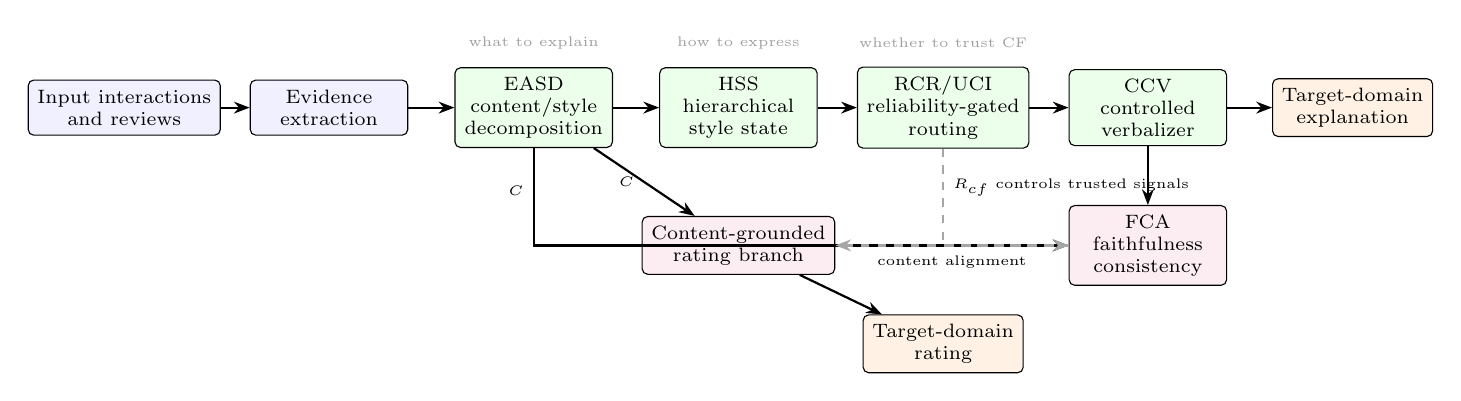
\begin{tikzpicture}[
  font=\scriptsize,
  module/.style={draw, rounded corners=2pt, align=center, minimum width=2.0cm, minimum height=0.7cm, fill=blue!6},
  core/.style={draw, rounded corners=2pt, align=center, minimum width=2.0cm, minimum height=0.7cm, fill=green!8},
  output/.style={draw, rounded corners=2pt, align=center, minimum width=2.0cm, minimum height=0.7cm, fill=orange!10},
  branch/.style={draw, rounded corners=2pt, align=center, minimum width=2.0cm, minimum height=0.65cm, fill=purple!7},
  arrow/.style={-{Stealth[length=2mm]}, thick},
  soft/.style={-{Stealth[length=2mm]}, thick, dashed, draw=gray!70}
]
\node[module] (Input) at (0,0) {Input interactions\\and reviews};
\node[module] (Evidence) at (2.6,0) {Evidence\\extraction};
\node[core] (EASD) at (5.2,0) {EASD\\content/style\\decomposition};
\node[core] (HSS) at (7.8,0) {HSS\\hierarchical\\style state};
\node[core] (RCR) at (10.4,0) {RCR/UCI\\reliability-gated\\routing};
\node[core] (CCV) at (13.0,0) {CCV\\controlled\\verbalizer};
\node[output] (Exp) at (15.6,0) {Target-domain\\explanation};

\node[branch] (Rating) at (7.8,-1.75) {Content-grounded\\rating branch};
\node[branch] (FCA) at (13.0,-1.75) {FCA\\faithfulness\\consistency};
\node[output] (RateOut) at (10.4,-3.0) {Target-domain\\rating};

\draw[arrow] (Input) -- (Evidence);
\draw[arrow] (Evidence) -- (EASD);
\draw[arrow] (EASD) -- (HSS);
\draw[arrow] (HSS) -- (RCR);
\draw[arrow] (RCR) -- (CCV);
\draw[arrow] (CCV) -- (Exp);
\draw[arrow] (EASD) -- node[left, font=\tiny] {$C$} (Rating);
\draw[arrow] (Rating) -- (RateOut);
\draw[arrow] (EASD) |- node[pos=0.22, left, font=\tiny] {$C$} (FCA);
\draw[arrow] (CCV) -- (FCA);
\draw[soft] (FCA) -- node[below, font=\tiny] {content alignment} (Rating);
\draw[soft] (RCR) |- node[pos=0.2, right, font=\tiny] {$R_{cf}$ controls trusted signals} (FCA);
\node[font=\tiny, text=gray!75] at (5.2,0.82) {what to explain};
\node[font=\tiny, text=gray!75] at (7.8,0.82) {how to express};
\node[font=\tiny, text=gray!75] at (10.4,0.82) {whether to trust CF};
\end{tikzpicture}
}
  \caption{ODCR overall architecture. The method maps input interactions and reviews into evidence extraction, EASD content/style decomposition, HSS hierarchical style state modeling, RCR/UCI reliability-gated counterfactual routing, CCV controlled explanation generation, and FCA faithfulness consistency. The content-grounded rating branch is separated from explanation generation while sharing content evidence.}
  \label{fig:overall_architecture}
\end{figure}

Figure~\ref{fig:overall_architecture} shows the resulting architecture. ODCR
does not ask one representation to absorb every textual factor. Instead, it
uses \(C\), \(S^{(t)}\), and \(R_{cf}\) as method-level controls for content,
expression, and counterfactual trust.

\subsection{Evidence-Anchored Content/Style Decomposition}

Evidence-Anchored Content/Style Decomposition (EASD) is the first ODCR module.
It separates stable content evidence from expression style while keeping both
anchored to observable user--item evidence. Content evidence \(C\) is tied to
rating-relevant aspects and interaction evidence. Style evidence captures
domain phrasing, emphasis, and lexical conventions that affect how content is
verbalized.

The key distinction is that ODCR does not leave shared and specific
representations to infer this split without guidance. The decomposition is
anchored: content is constrained by preference evidence, while style is
constrained by domain-specific expression signals. This turns the coarse
attribute \(W^{(t)}\) into a controllable pair: \(C\) determines what should be
explained, and \(S^{(t)}\) determines how that evidence is expressed. Rating
prediction and explanation generation can therefore share content evidence
without collapsing explanation style into the rating branch.

\subsection{Hierarchical Style State}

Hierarchical Style State (HSS) models style as more than a domain identifier.
ODCR writes the style state as
\[
  S^{(t)} = \bigl(S_{\mathrm{domain}}^{(t)}, \Delta S_{\mathrm{local}}^{(t)}\bigr),
\]
where \(S_{\mathrm{domain}}^{(t)}\) captures domain-global textual conventions
and \(\Delta S_{\mathrm{local}}^{(t)}\) captures instance-local residual style.
The domain component models broad conventions such as review tone and
domain-common phrasing. The local residual captures user--item-specific
stylistic variation that should not be forced into a single domain template.

HSS makes the D4C feedback channel more precise. If explanations feed back
into the future textual environment, ODCR localizes that feedback mainly to
\(S^{(t+1)}\). Content evidence \(C\) should remain a stable anchor for what is
being recommended and explained. This prevents dynamic feedback from
corrupting content while still allowing expression style to evolve with the
target domain.

\subsection{Reliability-Gated Counterfactual Control}

Reliability-Gated Counterfactual Control combines RCR and uncertainty-aware
counterfactual invariance (UCI). D4C shows that counterfactual domain evidence
can reduce shortcut dependence, but ODCR further recognizes that
counterfactual examples are not equally trustworthy. Some preserve content and
shift only style; others alter the recommendation evidence or introduce noisy
signals.

ODCR uses two control layers. The first layer is eligibility filtering: a
counterfactual example is usable only if it preserves the content needed for
the target explanation and does not violate the intended transfer setting. The
second layer is reliability weighting and sampling priority: usable
counterfactual examples receive different influence according to \(R_{cf}\)
and uncertainty. A compact module-level objective is
\[
  \mathcal{L}_{\mathrm{ODCR}}
  =
  \mathcal{L}_{\mathrm{fact}}
  +
  \lambda \sum_j R_{cf,j}\,\mathcal{L}_{\mathrm{cf},j},
\]
where \(\mathcal{L}_{\mathrm{fact}}\) is factual learning, \(\mathcal{L}_{\mathrm{cf},j}\)
is the counterfactual learning signal for candidate \(j\), and \(R_{cf,j}\)
controls its influence. UCI reduces trust in unstable or uncertain
counterfactual signals rather than treating every counterfactual example as
equally informative.

\begin{figure}[t]
  \centering
  \resizebox{\textwidth}{!}{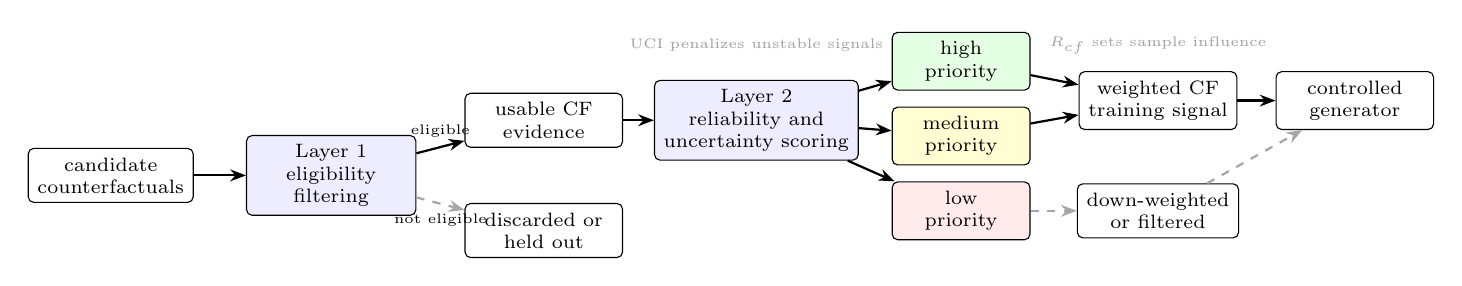
\begin{tikzpicture}[
  font=\scriptsize,
  box/.style={draw, rounded corners=2pt, align=center, minimum width=2.0cm, minimum height=0.65cm, fill=white},
  gate/.style={draw, rounded corners=2pt, align=center, minimum width=2.15cm, minimum height=0.7cm, fill=blue!7},
  high/.style={draw, rounded corners=2pt, align=center, minimum width=1.75cm, minimum height=0.6cm, fill=green!10},
  med/.style={draw, rounded corners=2pt, align=center, minimum width=1.75cm, minimum height=0.6cm, fill=yellow!18},
  low/.style={draw, rounded corners=2pt, align=center, minimum width=1.75cm, minimum height=0.6cm, fill=red!8},
  arrow/.style={-{Stealth[length=2mm]}, thick},
  dline/.style={-{Stealth[length=2mm]}, thick, dashed, draw=gray!70}
]
\node[box] (CF) at (0,0) {candidate\\counterfactuals};
\node[gate] (Elig) at (2.8,0) {Layer 1\\eligibility\\filtering};
\node[box] (Use) at (5.5,0.7) {usable CF\\evidence};
\node[box] (Drop) at (5.5,-0.7) {discarded or\\held out};
\node[gate] (Score) at (8.2,0.7) {Layer 2\\reliability and\\uncertainty scoring};
\node[high] (High) at (10.8,1.45) {high\\priority};
\node[med] (Med) at (10.8,0.5) {medium\\priority};
\node[low] (Low) at (10.8,-0.45) {low\\priority};
\node[box] (Train) at (13.3,0.95) {weighted CF\\training signal};
\node[box] (Filter) at (13.3,-0.45) {down-weighted\\or filtered};
\node[box] (Gen) at (15.8,0.95) {controlled\\generator};

\draw[arrow] (CF) -- (Elig);
\draw[arrow] (Elig) -- node[above, font=\tiny] {eligible} (Use);
\draw[dline] (Elig) -- node[below, font=\tiny] {not eligible} (Drop);
\draw[arrow] (Use) -- (Score);
\draw[arrow] (Score) -- (High);
\draw[arrow] (Score) -- (Med);
\draw[arrow] (Score) -- (Low);
\draw[arrow] (High) -- (Train);
\draw[arrow] (Med) -- (Train);
\draw[dline] (Low) -- (Filter);
\draw[arrow] (Train) -- (Gen);
\draw[dline] (Filter) -- (Gen);
\node[font=\tiny, text=gray!75] at (8.2,1.65) {UCI penalizes unstable signals};
\node[font=\tiny, text=gray!75] at (13.3,1.65) {$R_{cf}$ sets sample influence};
\end{tikzpicture}
}
  \caption{RCR/UCI routing mechanism. Counterfactual candidates first pass eligibility filtering, then receive reliability and uncertainty-aware weights that determine sampling priority and training influence. Low-reliability evidence is down-weighted or filtered rather than treated as equal counterfactual supervision.}
  \label{fig:rcr_routing}
\end{figure}

Figure~\ref{fig:rcr_routing} illustrates this two-layer routing mechanism. The
figure is intended as a method diagram and as an insertion point for later
module ablations; it does not claim that a complete ablation suite is already
integrated into the current result tables.

\subsection{Controlled Causal Verbalizer and Faithfulness Alignment}

The Controlled Causal Verbalizer (CCV) is the output-side module. Instead of
learning the shortcut \(P(E\mid W)\), ODCR conditions explanation generation on
the refined variables:
\[
  P(E \mid U, I, C, S, R_{cf}) .
\]
Content evidence \(C\) controls what should be said, style state \(S\) controls
how it should be expressed, and \(R_{cf}\) controls which counterfactual
training signals are trusted. This design makes explanation generation a
controlled causal verbalization problem rather than an unconstrained
domain-language imitation problem.

Faithfulness Consistency Alignment (FCA) keeps the generated explanation tied
to content-grounded recommendation evidence. Style transfer should not
substitute for preference evidence, and a fluent target-domain explanation
should not drift away from the aspects that support the rating branch. FCA is
therefore the consistency principle linking CCV back to \(C\): the output may
adapt its expression style, but its content should remain aligned with
rating-relevant evidence.

\subsection{Implementation Mapping}

The implementation maps these method modules to the current ODCR workflow
without making workflow stages the paper's primary contribution. Preprocessing
and Step3 support EASD/HSS by preparing evidence and learning content/style
representations. Step4 supports RCR/UCI through reliability estimation,
routing, confidence buckets, uncertainty signals, and sample-weight hints.
Step5\_e supports CCV/FCA as explanation-only controlled generation. Rating
evidence remains content-grounded and separate from explanation generation,
while explanation learning consumes reliability-gated evidence for target-domain
verbalization.

\section{Experimental Setup}

\subsection{Datasets and Directed Transfer Settings}

The reset table system evaluates three Amazon target-domain settings. For
AM-CDs, AM-Electronics and AM-Movies are used as auxiliary domains. For
AM-Electronics, AM-CDs and AM-Movies are used as auxiliary domains. For
AM-Movies, AM-CDs and AM-Electronics are used as auxiliary domains. In each
setting, the target dataset is the evaluation dataset, and the auxiliary domain
is the source of cross-domain transfer signal.

\subsection{Metrics}

We report automatic text-generation metrics and rating-error metrics in the
same overall performance tables. The text metrics are ROUGE-1, ROUGE-L, BLEU-1,
BLEU-2, BLEU-3, BLEU-4, METEOR, DIST-1, and DIST-2. Rating errors are reported
by RMSE and MAE. Larger values are better for the automatic text metrics, while
smaller values are better for RMSE and MAE.

\subsection{Baselines and Comparison Scope}

The main tables follow the D4C-style comparison format. Single-domain
baselines are DualPC, PETER, ReXPlug, and ERRA. Cross-domain baselines are
PEFT, PEPLER, AdaReX, and D4C. Our method is reported as ReCEG in the result
tables. D4C is the closest causal reference point for the dynamic
textual-feedback view \cite{d4c}. Classical explainable recommendation systems
are cited as task-family context where appropriate \cite{peter,pepler,adarex}.

\subsection{Evaluation Scope}

We report current results on three Amazon target-domain settings. The baseline
rows follow D4C-style reporting, but standard deviations are omitted for
compactness. The results should be read as bounded evidence rather than as a
multi-seed benchmark claim.

\section{Results}

\subsection{Overall Performance on AM-CDs}

\begin{table*}[t]
\centering
\caption{Overall Performance on the AM-CDs Dataset}
\scriptsize
\setlength{\tabcolsep}{2.5pt}
\resizebox{\textwidth}{!}{%
\begin{tabular}{lrrrrrrrrrrr}
\toprule
Methods & ROUGE-1 & ROUGE-L & BLEU-1 & BLEU-2 & BLEU-3 & BLEU-4 & METEOR & DIST-1 & DIST-2 & RMSE & MAE \\
\midrule
\multicolumn{12}{l}{\textit{Single Domain}} \\
DualPC & 12.50 & 9.67 & 9.32 & 3.69 & 1.60 & 0.88 & 7.98 & 0.01 & 0.02 & 0.9563 & 0.6736 \\
PETER & 11.62 & 9.07 & 10.42 & 3.86 & 1.77 & 0.99 & 8.41 & 0.78 & 2.64 & 0.9191 & 0.6577 \\
ReXPlug & 13.16 & 10.18 & 9.85 & 3.86 & 1.64 & 0.88 & 8.13 & 0.59 & 2.53 & 0.9580 & 0.6751 \\
ERRA & 12.72 & 9.92 & 11.53 & 4.32 & 1.99 & 1.12 & 8.88 & 0.42 & 1.46 & 0.9128 & 0.6592 \\
\midrule
\multicolumn{12}{l}{\textit{Cross-Domain}} \\
PEFT (E) & 12.37 & 9.57 & 11.68 & 4.34 & 2.00 & 1.13 & 9.17 & 0.83 & 2.88 & 0.9091 & 0.6653 \\
PEFT (M) & 12.41 & 9.69 & 11.67 & 4.29 & 1.95 & 1.10 & 8.98 & 0.53 & 1.75 & 0.9050 & 0.6767 \\
PEPLER (E) & 12.59 & 9.78 & 11.57 & 4.08 & 1.79 & 0.98 & 8.87 & 0.80 & 3.21 & 0.9008 & 0.6561 \\
PEPLER (M) & 12.80 & 9.71 & 11.67 & 4.07 & 1.78 & 0.97 & 8.94 & 0.70 & 2.94 & \textbf{0.9003} & 0.6568 \\
AdaReX (E) & 13.42 & 10.37 & 12.64 & 4.54 & 2.00 & 1.08 & 9.48 & 0.67 & 2.62 & 0.9188 & \textbf{0.6505} \\
AdaReX (M) & 13.38 & 10.40 & 12.60 & 4.67 & 2.09 & 1.15 & 9.52 & 0.89 & 3.13 & 0.9178 & 0.6582 \\
D4C (E) & 13.50 & 10.61 & 12.71 & 4.69 & 2.23 & 1.21 & 9.69 & 0.93 & 3.57 & 0.9130 & 0.6594 \\
D4C (M) & 13.41 & 10.49 & 12.84 & 4.85 & 2.29 & 1.26 & 9.82 & 0.98 & 4.07 & 0.9179 & 0.6601 \\
ReCEG (E) & \textbf{14.02} & \textbf{10.98} & 13.06 & 4.98 & 2.40 & 1.34 & 10.12 & 1.04 & 4.28 & 0.9010 & \textbf{0.6505} \\
ReCEG (M) & 13.94 & 10.89 & \textbf{13.20} & \textbf{5.10} & \textbf{2.49} & \textbf{1.41} & \textbf{10.24} & \textbf{1.09} & \textbf{4.55} & 0.9030 & 0.6515 \\
\bottomrule
\end{tabular}%
}
\vspace{2pt}
\parbox{\textwidth}{\scriptsize \textit{Note:} ``E'' and ``M'' refer to AM-Electronics and AM-Movies as the auxiliary domains, respectively. Bold values indicate the best performance.}
\label{tab:overall_performance_am_cds}
\end{table*}


Table~\ref{tab:overall_performance_am_cds} reports AM-CDs as the target
dataset with AM-Electronics and AM-Movies as auxiliary domains. The table uses
the full D4C-style baseline set, separating single-domain methods from
cross-domain methods. ReCEG improves over the corresponding D4C rows on all
text-generation metrics for both auxiliary domains. The auxiliary domains show
different strengths: ReCEG with AM-Electronics is stronger on ROUGE-1,
ROUGE-L, and rating error among the ReCEG rows, while ReCEG with AM-Movies is
stronger on BLEU, METEOR, and diversity.

\subsection{Overall Performance on AM-Electronics}

\begin{table*}[t]
\centering
\caption{Overall Performance on the AM-Electronics Dataset}
\scriptsize
\setlength{\tabcolsep}{2.5pt}
\resizebox{\textwidth}{!}{%
\begin{tabular}{lrrrrrrrrrrr}
\toprule
Methods & ROUGE-1 & ROUGE-L & BLEU-1 & BLEU-2 & BLEU-3 & BLEU-4 & METEOR & DIST-1 & DIST-2 & RMSE & MAE \\
\midrule
\multicolumn{12}{l}{\textit{Single Domain}} \\
DualPC & 10.43 & 8.13 & 9.79 & 2.62 & 0.81 & 0.35 & 7.61 & 0.01 & 0.02 & 1.1018 & 0.7876 \\
PETER & 12.68 & 9.55 & 12.04 & 3.87 & 1.44 & 0.65 & 8.89 & 0.64 & 2.00 & 1.0550 & 0.7618 \\
ReXPlug & 10.83 & 8.69 & 9.36 & 2.76 & 0.85 & 0.30 & 7.93 & 0.53 & 1.11 & 1.0868 & 0.7809 \\
ERRA & 13.27 & 10.01 & 13.25 & 4.30 & 1.56 & 0.69 & 9.55 & 0.64 & 2.04 & 1.0506 & \textbf{0.7577} \\
\midrule
\multicolumn{12}{l}{\textit{Cross-Domain}} \\
PEFT (C) & 12.67 & 9.41 & 12.04 & 3.85 & 1.43 & 0.62 & 8.87 & 0.69 & 1.29 & 1.0459 & 0.7727 \\
PEFT (M) & 12.89 & 10.01 & 13.85 & 4.20 & 1.32 & 0.54 & 9.53 & 0.33 & 1.07 & 1.0508 & 0.7679 \\
PEPLER (C) & 14.01 & 10.09 & 12.48 & 3.87 & 1.36 & 0.54 & 10.29 & 0.24 & 1.21 & \textbf{1.0348} & 0.7657 \\
PEPLER (M) & 13.91 & 10.47 & 12.45 & 3.85 & 1.37 & 0.55 & 10.26 & 0.25 & 1.22 & 1.0349 & 0.7661 \\
AdaReX (C) & 13.27 & 9.98 & 13.11 & 4.25 & 1.53 & 0.66 & 9.60 & 0.50 & 1.63 & 1.0662 & 0.7771 \\
AdaReX (M) & 13.53 & 9.70 & 13.44 & 3.98 & 1.43 & 0.57 & 9.42 & 0.55 & 1.87 & 1.0622 & 0.7726 \\
D4C (C) & 14.02 & 10.42 & 14.16 & 4.39 & 1.69 & 0.78 & 10.32 & 0.68 & 2.21 & 1.0847 & 0.7836 \\
D4C (M) & 13.56 & 10.19 & 13.58 & 4.33 & 1.68 & 0.79 & 10.24 & 0.85 & 2.39 & 1.0794 & 0.7756 \\
ReCEG (C) & \textbf{14.38} & \textbf{10.68} & \textbf{14.50} & \textbf{4.58} & 1.82 & 0.88 & \textbf{10.65} & 0.76 & 2.54 & 1.0710 & 0.7710 \\
ReCEG (M) & 13.96 & 10.48 & 13.96 & 4.51 & \textbf{1.83} & \textbf{0.89} & 10.55 & \textbf{0.94} & \textbf{2.76} & 1.0660 & 0.7675 \\
\bottomrule
\end{tabular}%
}
\vspace{2pt}
\parbox{\textwidth}{\scriptsize \textit{Note:} ``C'' and ``M'' refer to AM-CDs and AM-Movies as the auxiliary domains, respectively. Bold values indicate the best performance.}
\label{tab:overall_performance_am_electronics}
\end{table*}


Table~\ref{tab:overall_performance_am_electronics} reports AM-Electronics as
the target dataset. ReCEG is strongest on the explanation-oriented columns:
ReCEG with AM-CDs leads ROUGE-1, ROUGE-L, BLEU-1, BLEU-2, and METEOR, while
ReCEG with AM-Movies leads BLEU-3, BLEU-4, DIST-1, and DIST-2. The best
rating-error values still come from earlier baselines in this table, which
keeps the evidence focused on explanation generation rather than recommendation
prediction. This split is consistent with the paper's content/style/reliability
story: one auxiliary domain contributes closer textual relatedness, while the
other contributes stronger diversity.

\subsection{Overall Performance on AM-Movies}

\begin{table*}[t]
\centering
\caption{Overall Performance on the AM-Movies Dataset}
\scriptsize
\setlength{\tabcolsep}{2.5pt}
\resizebox{\textwidth}{!}{%
\begin{tabular}{lrrrrrrrrrrr}
\toprule
Methods & ROUGE-1 & ROUGE-L & BLEU-1 & BLEU-2 & BLEU-3 & BLEU-4 & METEOR & DIST-1 & DIST-2 & RMSE & MAE \\
\midrule
\multicolumn{12}{l}{\textit{Single Domain}} \\
DualPC & 11.83 & 9.10 & 9.21 & 3.04 & 1.23 & 0.63 & 7.94 & 0.03 & 0.06 & 1.0504 & 0.7567 \\
PETER & 14.35 & 10.92 & 13.24 & 4.82 & 2.18 & 1.21 & 9.75 & 0.48 & 1.85 & 0.9959 & 0.7411 \\
ReXPlug & 10.86 & 8.30 & 6.83 & 2.10 & 0.72 & 0.30 & 6.55 & 0.39 & 1.37 & 1.0236 & 0.7479 \\
ERRA & 13.71 & 10.47 & 12.14 & 4.41 & 1.99 & 1.14 & 9.42 & 0.33 & 1.26 & 1.0025 & 0.7413 \\
\midrule
\multicolumn{12}{l}{\textit{Cross-Domain}} \\
PEFT (C) & 13.79 & 9.93 & 12.24 & 4.72 & 1.90 & 1.05 & 9.56 & 0.57 & 2.23 & 0.9944 & 0.7339 \\
PEFT (E) & 13.89 & 9.97 & 12.22 & 4.90 & 1.88 & 1.04 & 10.14 & 0.45 & 1.59 & 0.9921 & 0.7471 \\
PEPLER (C) & 13.66 & 11.20 & 12.80 & 5.25 & 2.20 & 1.29 & 10.21 & 0.59 & 2.98 & \textbf{0.9919} & 0.7598 \\
PEPLER (E) & 13.62 & 10.52 & 12.65 & 4.94 & 2.23 & 1.17 & 10.13 & 0.61 & 3.01 & 0.9920 & 0.7598 \\
AdaReX (C) & 13.97 & 10.60 & 12.53 & 4.62 & 2.11 & 1.20 & 9.94 & 0.44 & 2.29 & 0.9987 & 0.7305 \\
AdaReX (E) & 14.21 & 10.89 & 13.31 & 4.81 & 2.11 & 1.23 & 9.97 & 0.52 & 2.24 & 0.9988 & 0.7360 \\
D4C (C) & 14.45 & 11.08 & 13.41 & 4.95 & 2.26 & 1.31 & 10.19 & 1.09 & 4.30 & 1.0045 & 0.7352 \\
D4C (E) & 14.54 & 11.25 & 13.49 & 5.12 & 2.33 & 1.30 & 10.13 & 0.98 & 3.97 & 1.0071 & 0.7376 \\
ReCEG (C) & 14.90 & 11.42 & 13.78 & 5.22 & 2.47 & \textbf{1.44} & \textbf{10.48} & \textbf{1.18} & \textbf{4.72} & 0.9960 & \textbf{0.7290} \\
ReCEG (E) & \textbf{14.98} & \textbf{11.55} & \textbf{13.88} & \textbf{5.34} & \textbf{2.53} & 1.43 & 10.45 & 1.10 & 4.46 & 0.9980 & 0.7310 \\
\bottomrule
\end{tabular}%
}
\vspace{2pt}
\parbox{\textwidth}{\scriptsize \textit{Note:} ``C'' and ``E'' refer to AM-CDs and AM-Electronics as the auxiliary domains, respectively. Bold values indicate the best performance.}
\label{tab:overall_performance_am_movies}
\end{table*}


Table~\ref{tab:overall_performance_am_movies} reports AM-Movies as the target
dataset. ReCEG with AM-Electronics is strongest on ROUGE and BLEU-1 through
BLEU-3, matching the stronger textual relatedness visible in the D4C rows.
ReCEG with AM-CDs is strongest on BLEU-4, METEOR, DIST-1, DIST-2, and MAE,
preserving the higher-diversity pattern associated with the AM-CDs auxiliary
domain. As in the other target-domain tables, explanation metrics show clearer
movement than rating-error metrics.

\subsection{Ablation Study on AM-CDs}

\begin{table*}[t]
\centering
\caption{Performance Comparison of Variants of Our Framework on the AM-CDs Dataset}
\small
\setlength{\tabcolsep}{6pt}
\resizebox{\textwidth}{!}{%
\begin{tabular}{lrrrrr}
\toprule
Methods & BLEU-3 & BLEU-4 & METEOR & DIST-1 & DIST-2 \\
\midrule
\multicolumn{6}{l}{\textit{AM-Electronics auxiliary domain}} \\
Original & 2.23 & 1.21 & 9.69 & 0.93 & 3.57 \\
ReCEG (w/o SE, w/o RG) & 2.15 & 1.16 & 9.55 & 0.87 & 3.25 \\
ReCEG (w/ SE, w/o RG) & \underline{2.29} & \underline{1.27} & \underline{9.89} & 0.90 & 3.43 \\
ReCEG (w/o SE, w/ RG) & 2.21 & 1.19 & 9.75 & \underline{0.98} & \underline{3.82} \\
ReCEG & \textbf{2.40} & \textbf{1.34} & \textbf{10.12} & \textbf{1.04} & \textbf{4.28} \\
\midrule
\multicolumn{6}{l}{\textit{AM-Movies auxiliary domain}} \\
Original & 2.29 & 1.26 & 9.82 & 0.98 & 4.07 \\
ReCEG (w/o SE, w/o RG) & 2.20 & 1.18 & 9.64 & 0.90 & 3.70 \\
ReCEG (w/ SE, w/o RG) & \underline{2.38} & \underline{1.34} & \underline{10.02} & 0.96 & 4.04 \\
ReCEG (w/o SE, w/ RG) & 2.28 & 1.25 & 9.88 & \underline{1.03} & \underline{4.31} \\
ReCEG & \textbf{2.49} & \textbf{1.41} & \textbf{10.24} & \textbf{1.09} & \textbf{4.55} \\
\bottomrule
\end{tabular}%
}
\vspace{2pt}
\parbox{\textwidth}{\scriptsize \textit{Note:} SE denotes Semantic Evidence modeling, and RG denotes Reliability Guidance. Underlined values indicate the best results among the three ReCEG variants excluding the full model; bold values indicate the overall best performance.}
\label{tab:ablation_am_cds}
\end{table*}


Table~\ref{tab:ablation_am_cds} studies the effect of semantic evidence
modeling and reliability guidance on the AM-CDs target setting. Removing both
components yields the weakest ReCEG variant. Adding semantic evidence improves
BLEU-3, BLEU-4, and METEOR, suggesting that evidence-aware content modeling
mainly strengthens explanation quality. Adding reliability guidance improves
DIST-1 and DIST-2, indicating that reliability-guided counterfactual use helps
reduce repetitive generation and improves diversity. The full model achieves
the best performance in both auxiliary-domain blocks, showing that semantic
evidence and reliability guidance are complementary.

\subsection{Discussion of the Results}

Across the three tables, ReCEG consistently improves explanation metrics over
D4C while retaining explicit RMSE and MAE reporting. The metric pattern is not
homogeneous across auxiliary domains, and that difference is important. AM-CDs
separates lexical/rating behavior from BLEU/diversity behavior across the two
auxiliary domains. AM-Electronics separates lexical relevance from diversity.
AM-Movies shows a parallel split, with AM-Electronics stronger on ROUGE/BLEU
and AM-CDs stronger on diversity and MAE. Together with the AM-CDs ablation in
Table~\ref{tab:ablation_am_cds}, these results support the manuscript as
bounded current evidence for the content/style/reliability framing, not as a
state-of-the-art or statistical significance claim.

\section{Discussion}

\subsection{Dynamic Feedback Control}

ODCR treats explanation degeneration as a dynamic causal-control problem. D4C's
feedback view explains why domain textual shortcuts can become
self-reinforcing: \(W^{(t)}\) influences explanations, and explanations can
feed back into \(W^{(t+1)}\). ODCR does not discard this diagnosis. It refines
the feedback loop so that stable content evidence, dynamic style, and
counterfactual reliability are controlled separately.

\subsection{Role of EASD and HSS}

EASD and HSS are the parts of ODCR that keep the paper from becoming centered
on reliability routing alone. EASD anchors content/style decomposition in evidence, separating what
should be explained from how it is expressed. HSS makes style feedback
hierarchical, with domain-global style and instance-local residuals. Together,
they define where dynamic feedback should operate: generated explanations may
reshape style, but they should not overwrite content evidence.

\subsection{Role of RCR/UCI and CCV/FCA}

RCR/UCI controls counterfactual influence after decomposition. It filters
counterfactual candidates, scores reliability, and uses uncertainty to reduce
trust in unstable shifts. CCV/FCA then turns the controlled evidence into
target-domain explanations. CCV conditions generation on \(U\), \(I\), \(C\),
\(S\), and \(R_{cf}\); FCA keeps explanation content aligned with
content-grounded rating evidence. This closes the ODCR loop from dynamic
feedback diagnosis to controlled faithful generation.

\subsection{Reading the Current Evidence}

The current result tables provide a compact main-text comparison over four
directed transfer settings. The Amazon blocks illustrate related-domain
content/style transfer, while the TripAdvisor--Yelp blocks place more stress on
style shift and reliability control. These results support the manuscript as
bounded current evidence. Additional ablations, human assessment, multi-seed
evaluation, and broader baseline adaptation can be integrated as later evidence
without changing the core method story.

\section{Limitations}

\paragraph{Evaluation scope.}
The current manuscript reports current ReCEG values in three Amazon
target-domain tables. The tables should not be interpreted as seed-robust
mean-and-standard-deviation estimates or as statistical-significance evidence.

\paragraph{Reference and benchmark compatibility.}
Strict longest-reference reconstruction and full D4C paper-compatible
benchmark reproduction are outside the present paper boundary. The current
tables are organized for compact method presentation, with baseline values
adapted from D4C-style reporting and ReCEG values shown as current bounded
evidence.

\paragraph{Broader baselines.}
Modern external baselines such as CIER, MAPLE, ELIXIR, Prism, and XRec require
same-setting adaptation before they can be used as result-table comparisons.
They are therefore discussed as comparison scope rather than as current result
claims.

\paragraph{Ablation scope.}
The current ablation table focuses on AM-CDs and on the two controls requested
for the main paper story: Semantic Evidence modeling and Reliability Guidance.
The manuscript therefore treats the ablation as table-supported evidence for
those controls, while avoiding broader component-isolation claims that would
require additional target-domain ablations.

\paragraph{Figure and presentation polish.}
The core method figures are now vector/TikZ diagrams intended for manuscript
review. Their visual density, placement, and AAAI camera-ready styling may
still need refinement after Chat review.

\section{Conclusion}

ODCR is presented as a reliability-gated dynamic causal refinement framework
for cross-domain explainable recommendation. Starting from D4C's feedback view
of explanation degeneration, ODCR refines coarse textual attributes
\(W^{(t)}\) into stable content evidence \(C\), feedback-sensitive hierarchical
style \(S^{(t)}\), and counterfactual reliability \(R_{cf}\). This reframing
turns cross-domain explanation learning into a controlled generation problem:
content determines what should be explained, style determines how it is
expressed, and reliability determines which counterfactual signals should
shape learning.

The resulting method loop combines EASD, HSS, RCR/UCI, and CCV/FCA. It keeps
rating evidence content-grounded while allowing the explanation generator to
adapt target-domain language without collapsing into a coarse textual shortcut.
The current tables provide bounded evidence on three Amazon target-domain
settings with different auxiliary-domain behavior. Future evidence additions
can extend this draft with module ablations, multi-seed evaluation, broader
baseline adaptation, and human or faithfulness-oriented assessment without
changing the central ODCR story.


\bibliographystyle{plain}
\bibliography{refs}

\end{document}
